\documentclass{article}


%Для мобилок
%\usepackage[left=20mm,right=20mm,top=20mm,bottom=20mm, paperwidth=150mm, paperheight=200mm]{geometry}


\usepackage{pgfplots}
\pgfplotsset{compat=1.9}
\pgfplotsset{major grid style={dashed,black}}
\pgfplotsset{minor grid style={solid,black}}
\usepackage{float}
%\usepackage{sidecap}
%\usepackage{csquotes} % ещё одна штука для цитат
\newtheorem{theorem}{Определение} % чтобы заработало окружение теорем

\usepackage[T2A]{fontenc}
\usepackage[utf8]{inputenc}
\usepackage[russian]{babel}
\usepackage{enumerate}
\usepackage{amsmath}

\newcommand{\rom}[1]
    {\MakeUppercase{\romannumeral #1}}

\usepackage{graphicx}
\title{Математический Анализ}
\author{Сахарова Нина Евгеньевна}
\begin{document}
\maketitle
 
\tableofcontents
 
 \section{Практика}
 \subsection{Организационное}
 \subsubsection{Модули и формула оценки}
 Курс - 2 года, \textbf{программа}(формулы оценки, информация о плане, контроле, полезной литературе, задачах для подготовке и т.п.) \textbf{на сайте}. Не все соответствует действительности - например, \textbf{учебники могут быть не те}. Но формулы точно ОК.
 
 Первые полгода  - \textbf{функция 1 переменной}. Вторые полгода - функции многих переменных. Третий семестр - \textbf{диффуравнения и т.п.}. Курс без лишнего формализма, теорем и доказательств. В первую очередь - практика. Кому захочется БДСМ - для вас \textbf{курс матфака}. Кому слишком жестко - \textbf{обращаться к Н.Е.}, поможет, даст задания, проконсультирует. Скорее всего, будет ОК.
 
 Формула оценки:
 $$
\begin{cases}
	Mark_{diploma} = Mark_1*0.25 + Mark_2*0.25 + Mark_3*0.25 + Mark_4*0.25
	\\
	Mark_1 = Mark_{exam}*0.3 + Mark_{kr}*0.3 + Mark_{dz+quiz}*0.4
	\\
	Mark_2 = Mark_{exam}*0.3 + Mark_{kr}*0.3 + Mark_{dz+quiz}*0.4
	\\
	Mark_3 = Mark_{exam}*0.3 + Mark_{kr}*0.3 + Mark_{dz+quiz}*0.4
	\\
	Mark_4 = Mark_{exam}*0.6 + Mark_{kr}*? + Mark_{dz+quiz}*?
\end{cases}
$$
 где \\
 $Mark_i$ - оценка за $i$-тый семестр \\
 $Mark_{exam}$ - оценка за экзамен \\
 $Mark_{kr}$ - контрольная в конце 1 модуля - начале 2го \\
 $Mark_{dz + quiz}$ - средняя оценка за дз и квизы aka самостоятельные.\\

 На кр можно шпору. Один лист в формате A4. С двух сторон. 	Домашняя - в \LaTeX, MS Word, или другом редакторе. \textbf{На паре иметь распечатку!} Дедлайны - святое. Если не будет - снижение оценки. Каждую неделю - листок с задачами. Он будет еще и в \textbf{Trello}. 
 \subsubsection{Правила}
\large{Низзя}
 \begin{itemize}
 \item{Списывать - будут нули у всех, у кого совпали работы, и не важно кто у кого списал.}
 \item{Стесняться на паре - будут проблемы на экзамене}
 \item{Сидеть в гаджетах. Конспекты в \LaTeX - можно :). Если все сильно срочно - ладно уж, можно.}
 \item{Изображать бревно, пока коллега у доски решает задачу. Решайте параллельно, а не списывайте с доски. Не ленитесь. Решайте задачи, это важно. Увидеть решение задачи другим человеком - недостаточно.}
 \item{Списывать задачи с Google}
 \item{Выпрашивать оценки в конце семестра(модуля)}
\item{Переписывать без уважительной причины. Без справки - фига вам. Все справки проверяются, если фальшивка - будут бить, и, возможно, ногами}
\item{Делать домашку не вовремя без уважительной причины}
\item{Писать на почту на ВШЭвском домене. \textbf{Она не читается.} Есть \textit{saharnina@gmail.com}}
\end{itemize}

Посещаемость не контролируется. Не ходите - ну и номрально, лишь бы сдавали все до дедлайнов. Но как показывает практика, лучше не бросать.
Вход-выход в/из аудитории - свободный. 
Учебники будут все в том же \textbf{Trello}. Дублирую тут:
\begin{itemize}
\item{Stewart?. Calculus. English only. Рекомендовано издание 2008 года. Читать как художественную литературу. Ссылочку дадут.}
\item{Классические учебники матана типа \textbf{Демидовича}. Ищите на свой вкус.}
\item{Моргунов. Будет в \textbf{Trello}.}
\item{...}
\item{Смотри \textbf{Trello}}
\subsubsection{Об экзамене}
У вас листок с задачами. Решаете их в течение 2-3 часов, со шпаргалкой, потом работы сдаются, проверяются, потом показа работ.
\end{itemize}

Первая неделя практика, без теории почти. Потом пойдет побольше теории. Пока вспоминаем школьное время: производная, интеграл.

\subsection{Лекция №1. Функция, производная.}

\subsubsection{Функции}
\begin{theorem}
Функция - такое отображение, при котором одному элементу числового множества соответствует \textbf{ровно один} элемент числового множества. Множество, откуда отображается - область определения $D_y$. То, куда - область занчений $E_y$.
\end{theorem}

Зависимость не обязана быть формулой, хоть это чаще всего и так. Переменных тоже может быть сколь угодно много.

\large{Способы задания:}
\begin{itemize}
\item{Таблицей}
\item{Формулой}
\item{Реккурентно - последовательности}
\item{Графиком}
\end{itemize}
В матанализе - в основном, применяются графики и формулы. Если на графике  есть возможноть провести вертикальную прямую так, чтобы она пересекла график дважды, то это \textbf{не функция}. Такой ужас задается двумя функциями: $x(t)$ и $y(t)$.	

Важные функции:
\begin{itemize}
\item{Линейная 

\begin{tikzpicture}
\begin{axis}[
	xlabel = {$x$},
	ylabel = {$y$},
	xmin=-5,
    xmax=5,
    ymin=-5,
    ymax=5,
    samples=1000,
     minor xtick = 0,
     minor ytick = 0,
	xtick = {-4,-2,...,4},
    ytick={-4,-2,...,4},
    grid=both,
    ]
\addplot[green] {x};
\addplot[black]{3*x+6};
\addplot[gray]{-2*x-6};
\addplot[blue]{-2*x+10};
\end{axis} 
\end{tikzpicture}
\begin{itemize}
\item{$y = kx + b$. $k$ - коэффициент наклона, чем больше,тем круче, $b$ - свободный член. Прямые задаются так все кроме вертикальной и горизонтальной.}
\item{$ax + by + c=0$ - тоже линейная функция.}
\item{Еще одна форма задания:$$\begin{cases}
y=at + c_1\\
x = bt + c_2
\end{cases}
$$

Параллельно вектору (a, b), смещено на вектор ($c_2, c_1$)
}
\item{
$$
\begin{cases}
y-y_0 = k(x - x_0)
\end{cases}
$$
}
\end{itemize}

}
\item{Степенные фукции. $y = x^n$
\begin{itemize}
\item{Квадратный трехчлен. 
$$\begin{cases}
y = ax^2 + bx +c\\
x_0 = \frac{-b}{2a}
\end{cases}$$

\begin{tikzpicture}
\begin{axis}[
	xlabel = {$x$},
	ylabel = {$y$},
	xmin=-20,
    xmax=20,
    ymin=0,
    ymax=40,
    samples=1000,
     minor xtick = 0,
     minor ytick = 0,
	xtick = {-20, -15,...,40},
    ytick = {0, 5,...,40},
    grid=both,
    ]
\addplot[red]{5*x^2 + 3*x + 6};
\addplot[green] {x^2};
\addplot[black]{-x^2 + 8};
\end{axis} 
\end{tikzpicture}
}

\item{Четные степени - параболы. 
$$y = ax^{2n}$$

\begin{tikzpicture}
\begin{axis}[
	xlabel = {$x$},
	ylabel = {$y$},
	xmin=-20,
    xmax=20,
    ymin=0,
    ymax=40,
    samples=5000,
     minor xtick = 0,
     minor ytick = 0,
	xtick = {-20, -15,...,40},
    ytick = {0, 5,...,40},
    grid=both,
    ]
\addplot[red]{x^2};
\addplot[green] {x^4};
\addplot[black]{-x^2 + 20};
\end{axis} 
\end{tikzpicture}
}


\item{Нечетные степени - кубические параболы. 
$$y = ax^{2n+1}$$

\begin{tikzpicture}
\begin{axis}[
	xlabel = {$x$},
	ylabel = {$y$},
	xmin=-10,
    xmax=10,
    ymin=-200,
    ymax=200,
    samples=1000,
     minor xtick = 0,
     minor ytick = 0,
	ytick = {-200, -165,...,200},
    xtick = {-10, -8,...,10},
    grid=both,
    ]
\addplot[red]{x^3};
\addplot[green] {1/100*x^5};
\end{axis} 
\end{tikzpicture}
}


\item{Отрицательные степени - гиперболы. 
$$y = ax^{-n}$$
\begin{tikzpicture}
\begin{axis}[
	xlabel = {$x$},
	ylabel = {$y$},
	ymin=-3,
    ymax=30,
    samples=1000,
    minor xtick = 0,
    minor ytick = 0,
	xtick = {-5, -4,...,5},
    ytick = {0, 4,...,50},
    grid=both,
    ]
\addplot[red]{1/x};
\end{axis} 
\end{tikzpicture}
}
\end{itemize}
}


\item{Полиноминальные функции
$$
y = \sum{a_ix^i}
\\
n_{extr} <= i_max
$$

\begin{tikzpicture}
\begin{axis}[
	xlabel = {$x$},
	ylabel = {$y$},
	ymin=-100,
    ymax=100,
    samples=1000,
    minor xtick = 0,
    minor ytick = 0,
	xtick = {-5, -4,...,5},
    ytick = {-75, -65,...,75},
    grid=both,
    ]
\addplot[red]{5*x^3 + 3*x^2 - 9*x + 6};
\addplot[red]{4*x^3 - 2*x^2 + 9*x - 3};
\end{axis} 
\end{tikzpicture}
}

\item{Рациональные
\begin{itemize}
\item{Показательные $y = a^x$. При $a<1$ - нисходящая, иначе - восходящая
\begin{tikzpicture}
\begin{axis}[
	xlabel = {$x$},
	ylabel = {$y$},
	ymin=-3,
    ymax=30,
    samples=1000,
    minor xtick = 0,
    minor ytick = 0,
	xtick = {-5, -4,...,5},
    ytick = {0, 4,...,50},
    grid=both,
    ]
\addplot[red]{e^x};
\addplot[green]{2^x};
\end{axis} 
\end{tikzpicture}
}
\item{Логарифмические $y = \log_a{x}$ . По определению, логарифм - обратная для экспоненты функция(см. ниже): 
$$
log_a{x}  = (a^x)^-1
$$

\begin{tikzpicture}
\begin{axis}[
	xlabel = {$x$},
	ylabel = {$y$},
	ymin=-3,
    ymax=30,
    samples=1000,
    minor xtick = 0,
    minor ytick = 0,
	xtick = {-5, -4,...,5},
    ytick = {0, 4,...,50},
    grid=both,
    ]
\addplot[red]{ln(x)};
\addplot[green]{ln(x)/ln(5)};
\end{axis} 
\end{tikzpicture}
Свойства:
\begin{itemize}
\item{$\log_a{b} + \log_a{c} = \log_a{b+c}$}
\item{$\log{a^b} = blog{a}$}
\end{itemize}
}
\end{itemize}
}
\end{itemize}

Композиция функций
$$f \circ g = f(g(x))$$

Пример:
$$
\begin{cases}
g(x) = \ln(x+2)
\\
f(x) = \sqrt{x+4}
\end{cases}
\\
f \circ f = \sqrt{ln(2+x) + 4}
$$

Функция называется обратной, если ${f^{-1}} \circ f = Eq$, где $Eq$ - тождественное отображение $Eq(x) = x$.

Пример: 
$$
f(x) = x^2
$$
$$
(x>0)
$$
$$
f^{-1} = \sqrt{x}
$$
$$
\sqrt{x^2} = x 
$$

Обратная функция является отражением относительно данной относительно оси $OX$. 

\begin{tikzpicture}
\begin{axis}[
    title = {$x^2$ и $\sqrt{x}$},
	xlabel = {$x$},
	ylabel = {$y$},
	xmin=0,
    xmax=5,
    ymin=0,
    ymax=5,
    samples=1000,
    ]
\addplot[green]{x};
\addplot[blue] {x^2};
\addplot[red] {sqrt(x)};
\end{axis} 
\end{tikzpicture}

\subsubsection{Пределы}

Допустим, у функции нет значения в некой точке $x_0$. Или это значение выдернуто:
$$
\begin{cases}
y=5x+3 (\forall x \neq 3)
\\
y=7 (x = 3)
\end{cases}
$$
Если мы хотим понять поведение этого около $x=3$, пишем следующее
$$\lim_{x \to x_0}{f(x)} = a$$
, что означает,что если мы берем числа, сколь угодно близкие к $x_0$, получаем числа, все более близкие к $a$.

\subsubsection{Производная}
Допустим, есть график движения материальной точки $S(t)$, и выбрано начало координат. Рассмотрим некое время $t_1$ и $t_2$. Проведем секущую, пересекающую функцию в точках $t_1$ и $t_2$. Скорость можно определить как $v=\frac{\Delta S}{ \Delta{t}}$. Устремив $\Delta t$ к нулю, получим мгновенную скорость и секущая станет касательной. Так и работает производная. Смотри ниже: на рисунке изображены именно такие касательные.

\begin{tikzpicture}
\begin{axis}[
	title = S(t),
	xlabel = {$t$},
	ylabel = {$S$},
	minor tick num = 2
]
\addplot[blue] {5*x^2 + 3*x + 6};
\addplot[red] {2*x+6};
\addplot[red] {2*x+7};
\addplot[red] {2*x+9};
\end{axis} 
\end{tikzpicture}

\subsection{Лекция №2.}

\subsubsection{Экстремумы и критические точки. Условия экстремума}

$f`(x) = lim_{\Delta x \to 0}\frac{f(x+\Delta x)}{\Delta x}$

Нули производной - критические точки, максимум или миниум - экстремум. Пример:
$x^3` = 3x^2$, но в нуле кубическая парабола экстремума не имеет:


\begin{tikzpicture}
\begin{axis}[
	title = S(t),
	xlabel = {$t$},
	ylabel = {$S$},
	minor tick num = 2
]
\addplot[blue] {x^3};
\end{axis} 
\end{tikzpicture}



Необходимо:
$$
\begin{cases}
f'(x_0)=0 or f'(x_0)  
\end{cases}
$$

Достаточно:
$$
\begin{cases}
f'(x_0)=0 or f'(x_0)
\\  
sgn(f'(x_0-dx)) = -sgn(f'(x_0+dx))
\end{cases}
$$

\subsection{Лекция №3.}
\subsubsection{Интеграл}

Пусть есть график зависимости скорости от времени. Требуется расчитать путь(найти площадь под графиком).

\begin{tikzpicture}
\begin{axis}[
xlabel = {$x$},
	ylabel = {$y$},
	ymin=-3,
    ymax=30,
    samples=1000,
    minor xtick = 0,
    minor ytick = 0,
	xtick = {-5, -4,...,5},
    ytick = {0, 4,...,50},
    grid=both,
    ]
]
\addplot[blue]{15};
\end{axis} 
\end{tikzpicture}

Путь - площадь прямоугольника, ограниченного следующими линиями:

$$
x=a
$$$$
x=b
$$$$
y=0
$$$$
y=v(t)
$$

Что же делать с нелинейной функцией? Делить на "ступеньки"! Чем больше ступенек, тем больше точность, а при устремлении их числа в $\infty$ получим точный ответ.

$$s = lim_{i \to \infty}\sum_{n=0}^iS_n = lim_{i \to \infty}\sum_{n=0}^if(x_n)\Delta n$$

где:
\\
$S_n = f(x_n)\Delta n$ - площадь $n$-ного прямоугольника
\\
$i$ - число прямоугольников

Эта сумма называется суммой Римана, кстати. Это будет определенный интеграл: 
$$S = \int^b_av(t)dt$$.

Сверху определние интеграла Римана, можно и по-другому.

Определнного интергала может и не существовать. Такие называются несобственными или расходящимися.

Рассмотрим путь как функцию от времени:
 $$S = \int^u_{a=const} v(t)dt = f(u) = S(u) - S(a)$$ 
Продифференцируем по $u$:
$$\frac{dS}{du} = \frac{dS(u)}{du} - \frac{dS(a)}{du} =  v(u) - 0$$

Мы только что показали, что производная и интеграл - взаимно обратные операции, хотя и не совсем формально и говорить так лучше не стоит.

Пусть $f(x) = \frac{dG}{dx}$, то есть $\Delta G = \Delta x f(x)$. 

Интеграл $\int^{b}_af(x)dx$ равен пределу Римановой суммы, с другой стороны, он равен $$\int^{b}_af(x)dx = \lim_{\Delta x \to 0}\sum\Delta G = G(b) - G(a)$$.
Это формула Ньютона-Лейбница, и она позволяет очень эффективно считать определенные интегралы, а не с пределами как в определении. 
 
Первообразная:


$$F(x) = \int f(x) dx <=> F'(x) = f(x)$$

! Первообразная определена с точностью до константы.

Условия существования обратной функции: $|D_y|=|E_y|$


\subsubsection{Дифференциал}
$$\Delta f(x) = f(x+\delta x) - f(x)$$
$$f'(x) =\lim _{\Delta x \to 0} \frac{\Delta f(x)}{\Delta x}$$
Далее говорим, что в пределе
$$\Delta f(x) = \Delta x * f'(x)$$
Или
$$df(x) = dx/f'(x) + \varepsilon$$
При этом $\varepsilon$ имеет порядок $dx^2$ или выше

Рассмотрим квадрат со стороной $x$. Его площадь, очевидно, $x^2$. Теперь увеличим сторону на $\Delta x$. Площадь стала $$(x+\Delta x)^2 = x^2 + 2x\Delta x + \Delta x^2 = x^2 + (x^2)'\Delta x + \Delta x^2$$. Ясно, что при малых $\Delta x$ порядок убывания $\Delta x^2$ выше, чем $\Delta x$ и он и есть тот самый $\varepsilon$ из уравнения выше.  

Ещё можно сказать,что $dy$ - изменение касательной к функции в данной точке за $dx$



\subsubsection{Как посчитать производную и интеграл}

\begin{enumerate}[I.]
\item{$$f(x) = Ag(x) + Bh(x) \Rightarrow
f'(x) = Ag'(x) + Bh'(x)$$
Докажем:
$$f'(x) = \lim_{\Delta x \to 0}\frac{\Delta f(x)}{\Delta x} = \lim_{\Delta x \to 0}\frac{A\Delta g(x) + B\Delta h(x))}{\Delta x} = Ag'(x) + Bh'(x) $$
}

\item{
$$\int f(x)+g(x)dx = \int f(x)dx + \int g(x)dx$$
Доказывается путем взятия производных от обоих частей. Действительно, производная от интеграла есть подынтегральная функция, и продифференцировав получим
$$f(x)+g(x) = f(x) + g(x)$$
}

\item{
Производная произведения

$$(f(x)*g(x))' = f'(x)*g(x) + g'(x)+f(x)$$

Докажем это:

$$f(x) = g(x)h(x)$$
$$\Delta f(x) = g(x+\Delta x)h(x + \Delta x) - g(x)h(x)$$
$$g+\Delta g = g(x+\Delta x)$$
$$\Delta f(x) = g\Delta h + h \Delta g + \Delta g \Delta h$$
$$\frac{\Delta f}{\Delta x} = g\frac{\Delta h}{\Delta x} + h\frac{\Delta g}{\Delta x} + \frac{\Delta g \Delta h}{\Delta x}$$
Последний член стремится к нулю при стремлении $\Delta x$ к нулю, то есть при переходе в пределы получим, что$$(f(x)*g(x))' = f'(x)*g(x) + g'(x)*f(x)$$
Что и требовалось доказать
}

\item{
Интегрирование по частям
$$(f(x)*g(x))' = f'(x)*g(x) + g'(x)+f(x)$$
Проинтегрировав это, получаем:
$$g(x)h(x)dx = f(x)\int g(x) + g(x)\int{h(x)}$$

Как использовать? Допустим, есть интеграл стостоящий из произведения двух функций, одна из которых легко интегрируется. Тогда можно сделать так:
$$\int g(x)f'(x) dx = f(x)g(x) - \int g'(x)f(x)$$
Например, 
$$\int xe^x = ?$$
Считаем $e^x = g', g=e^x, f = x, f'=1$

Тогда
$$\int xe^x = xe^x + \int e^x*1 dx = xe^x - e^x + C$$
}

\item{
Производная сложной функции. Рассмотрим $f(x)=g \circ h(x) = g(h(x))$
Рассмотрим $f$ как функцию $g$. 

Тогда $df = f'(g)*dg$. 

Но $dg = g'(x)*dx$

Из двух предыдущих получим

$$
df = f'(g)*g'(x)dx \Rightarrow f'(x) =  f'(g)*g'(x)
$$
}

\item{
Замена переменной в интергале aka Подведение под диференциал

Допустим, что
$$x = \phi(t) \Rightarrow dx = \phi'(t)dt$$
Тогда
$$\int f(x)dx = \int f(\phi(t))\phi'(t)dt$$

Пример:

$$\int 2xe^{x^2}dx =|t=x^2|= \int e^t dt = e^t + C= e^{x^2} + C$$

Или
 
$$\int 2xe^{x^2}dx = \int e^{x^2} 2xdx = \int e^{x^2}d(x^2) = |t=x^2| = \int e^t dt = e^t + C = e^{x^2} + C$$

}

\item{
Производная обратно функции
$$(f^{-1}(x))' = \frac{1}{f'(f^{-1}(x))}$$
}\begin{flushleft}\end{flushleft}
\end{enumerate}
\section{Нормальный матан}
\subsection{Множества и отображения. Числа}
\begin{theorem}
Множество - набор элементов, объединенный некоторым правилом.
\end{theorem}

Элементы множества  уникальны! Элементы перечисляются в фигурных скобках. Множества обозначаются заглавными латинскими буквами.

$$A = \{1,2,3,4,5,6 \}$$

Пустое множество - не содержит элементов $\empty$

Число элементов множества называют его \emph{мощностью} $|A|$ или $\#A$. У множества выше $\#A=6$.

Подмножество $B$ множества $A$ - такое множество, каждый элемент которого принадлежит $A$. Например, множество $B = {2,4,6} \subset A$

Операции:
$$A = \{1,2,3,4\}$$
$$B = \{3,4,5\}$$
\begin{itemize}
\item{
Объединение:
$$A\cup B = \{1,2,3,4,5\}$$
}
\item{
Исключение:
$$A \setminus B = \{1,2\}$$
}

\item{
Пересечение:
$$A\cap B = \{1,2,3,4,5\}$$
}


\item{
Симметрическая разность:
$$(A\setminus B) \cap (B\setminus A) = {1,2,5}$$
}


\item{
Декартово произведение
$$A*B = \{\{1,3\}, \{1,4\}, \{1,5\}, \{2,3\} ,\{2,4\},\{2,5\},\{3,3\},\{3,4\},\{3,5\},\{4,3\},\{4,4\},\{4,5\}\}$$
Пример такого - системы координат. Множество точек есть произвередние множеств $X$ и $Y$
}

\end{itemize}

Отображение $$f:A\to B$$ - это правило, сопоставляющее каждому элементу из $A$  элемент из $B$. Элементы из $A$ обязаны перейти куда-то, но элементы $B$ могут быть не затронуты. Образ элемента - то, во что он переходит. Прообраз - то,что переходит в данный элемент.

Композиция отображений - последовательное применение отображений к множеству. Пусть есть $f:A\to B$ и $g:B\to C$. Их комбинация отображение $f\circ g: A \to C$.

Биекция - взаимно однозначное отображение. Инъекция - такое отображение, при котором у любого элемента есть роно один образ. Сюрьекция - такое отображение, при котором у каждого элемента есть прообраз. Таким образом, Биекция - это Инъекция и Сюрьекция одновременно.

Если одно множество яляется подмножеством другого, это ничего не говорит об их мощности. Так, множества целых и натуральных чисел - равномощны. А вот множество действительных чисел больше. Доказательсто - смотри диагональный метод Кантора.

Обратимное отображение - такое отображение, что 
$$\begin{cases}
f\circ f^{-1}(b) = b
\\
f^{-1} \circ f (a) = a
\end{cases}$$

Оно существует только тогда, когда 

$$\begin{cases}
|B| = |A|
\\
f:A \to B - biection
\end{cases}$$

\section{Функции}

$ f(x): R\to R \Leftrightarrow f(x)=y, x \in R, y \in R $
\subsection{Про графики}
Модуль функции - отражение нижней части вверх отн. оси X; модуль аргумента - отражение правой части функции налево, <<затирая>> левую часть. Ниже: синяя - оригинальная функция, зеленая - модуль аргумента, красная - модуль функции.

\begin{tikzpicture}
\begin{axis}[
    xlabel = {$x$},
	ylabel = {$y$},
	ymin=-3,
    ymax=30,
    samples=1000,
    minor xtick = 0,
    minor ytick = 0,
	xtick = {-5, -4,...,5},
    ytick = {0, 4,...,50},
    grid=both,
    ]
]

\addplot[red]{abs(5*x^3-8*x^2+2*x+5)};
\addplot[green]{5*abs(x)^3-8*abs(x)^2+2*abs(x)+5};
\addplot[blue]{5*x^3-8*x^2+2*x+5};
\end{axis} 
\end{tikzpicture}

Сдвиг по аргументу: при замене $x \to kx+b$, функция сдвигается влево на b/k. При прибавлении к функции константы $C$, она сдвигается вверх на $C$. Синяя - оригинальная ф-ция, Красная - $f(x+C)$, зеленая - $f(x)+C$ 

\begin{tikzpicture}
\begin{axis}[
    xlabel = {$x$},
	ylabel = {$y$},
	ymin=-3,
    ymax=30,
    samples=1000,
    minor xtick = 0,
    minor ytick = 0,
	xtick = {-5, -4,...,5},
    ytick = {0, 4,...,50},
    grid=both,
    ]
]

\addplot[red]{5+(2*x^3-3*x^2+2*x+5)};
\addplot[blue]{2*x^3-3*x^2+2*x+5};
\addplot[green]{2*(x+5)^3-3*(x+5)^2+2*(x+5)+5};
\end{axis} 
\end{tikzpicture}

\subsection{Пределы функции}

По Коши:   
$$\lim_{x\to x_0} f(x) = A \Leftrightarrow \forall \varepsilon >0 \exists \delta >0: |x-x_0|<\delta \Rightarrow |f(x)-A| <\varepsilon $$

По Гейне: 
$$\lim_{x\to x_0} f(x) = A \Leftrightarrow \forall {a_n}: \lim a_n=x_0 \Rightarrow \lim f(a_n) = A $$


\subsubsection{Арифметика пределов}
Если $lim_{x\to x_0} f(x) = a$, $lim_{x\to x_0} g(x) = b$, $a,b \in R$
$$lim _{x\to x_0}(f(x)+g(x)) = a+b$$
$$lim _{x\to x_0}(f(x)-g(x)) = a-b$$
$$lim _{x\to x_0}(f(x)*g(x)) = a*b$$
$$lim _{x\to x_0}(f(x)/g(x)) = a/b$$

\subsubsection{Немного определений}

$$lim _{x\to x_0} F(x) = + \infty \Leftrightarrow \forall C \in R \exists \delta>0:|x-x_0|<\delta \Rightarrow f(x)>C$$
$$lim _{x\to \infty} = a \Leftrightarrow \forall \varepsilon>0 \exists C\in R: x>C \Rightarrow |f(x)-a|<\varepsilon$$

\subsubsection{Ассимптоты}

$x=a$ - вертикальная ассимптота, если $lim_{x\to a^+} f(x)=+-\infty$ или $lim_{x\to a^-} f(x)=+-\infty$

Если $f(x)$ имеет разные знаки в точках $a$ и $b$, при этом она непрерывна на $[a;b]$. Тогда у нее есть корень $c: f(c)=0$ на $[a;b]$



\subsubsection{Дифференциал}
Дифференциал функции - линейная часть ее приращения. Приращение функции $\Delta y = f(\Delta x) = k \Delta x + f(\Delta x^2)$. При $\Delta x \to 0$, линейный член вносит больший вклад, чем все другие. Дифференциал же равен просто $dy =k\Delta x$.

Пусть существует $$lim_{\Delta x \to 0}\frac{\Delta y}{\Delta x} = lim_{\Delta x \to 0}\frac{f(x_0 + \Delta x) - f(x_0)}{\Delta x} =f'(x)$$

Он называется \textbf{производной функции}. Кроме того, он имеет интересное соотношение с дифференциалом

$$dy = f'(x)\cdot dx$$


\subsection*{Ряды Тейлора}

Пусть функция $f(x)$ дифференцируема $n+1$ раз на отрезке от $x$ до $a$. Тогда найдется точка $\chi$, такая что 

$$f(x) = f(a) + \frac{f'(a)}{1!}(x-a) + \frac{f''(a)}{2!}(x-a)^2 + \frac{f^(n)(a)}{n!}x^n + R_n$$
$$R_n = o((x-a)^n)$$
$$R_n = f^{(n+1)(\chi)}{(n+1)!}(x-a)^{n+1}$$

$R_n$ - остаточный член в записи Пеано и Лагранжа соответственно.
\subsubsection*{Доказательства}

Докажем для формы Пеано. Пусть 
$$T_n(a) = f(a) + \frac{f'(a)}{1!} + \frac{f''(a)}{2!} + \frac{f^(n)(a)}{n!}$$
$$R_n(a) = f(a) - T_n(a) = 0$$
$$R_n'(a) = 0$$

$$\lim_{x \to a} \frac{R_n(x)}{(x-a)^n} = \lim_{x-a}\frac{R_n^{(n)}(x)}{n!} = 0$$

Докажем для формы Лагранжа.

$$f(x) = f(0) + \frac{f'(0)}{1!}x + \frac{f''(0)}{2!}x^2 + \frac{f^{(n)}(0)}{n!}x^n + \frac{f^{(n+1)}(0)}{n!}x^{n-1}$$
$$R_n^{(n+1)}(x) = f^{(n+1)}(x)$$

Применим теорему Коши к двум функциям: $R_n(x)$ и $F^{(n+1)}(x)$ на отрезке $(0,x)$. Существует такая точка, что 
$$\frac{R_n(x) - R_n(0)}{x^{n+1}} = \frac{R_n'(c_1)}{(n+1)c_1^n} \Rightarrow R_n(x) = R'_n(c_1){(n+1)c_1^n)}x^{n+1}$$

Снова теорема Коши. Существует такая точка $c_2$

$$\frac{R_n'(c_1) - r_n(0)}{c_1^n} = \frac{R_N''(c_2)}{nc_2^{n-1}}$$
$$\frac{R_n'(c_1)}{c_1^n} = \frac{R_N''(c_2)}{nc_2^{n-1}}$$

Применив ее $n$ раз, получим

$$r_n(x) = \frac{R_n^{(n)}c_n}{(n+1)!c_n}x^{n+1}$$

По теореме Лагранжа, существует точка $\chi$, такая что

$$\frac{R_n^{n}(c_n) - R_n^{(n)}(0)} = R_n^{(n+1)}(\chi) = f^{(n+1)}(\chi)$$

Объединив это с формулой выше, получим запись в форме Лагранжа.

\subsubsection*{Аппроксимация рядами тейлора}

$$f(x) = f(a) + \frac{f'(a)}{1!}x + \frac{f''(a)}{2!}x^2 + \frac{f^{(n)}(a)}{n!}x^n = \sum_{n=0}^{\inf} \frac{f^{(n)}(a)}{n!}x^n$$

Когда функция равна своему ряду тейлора? Какой долна быть $f(x)$ для выполнения формулы выше?

Представим ряд Тейлора как $T_n+R_n$ на промежутке $[a-r;a+r]$

Если существует константа $M$ такая что $|f^{(n)}(x)| \le M$ на $(a-r;a+r)$, то функция равна своему ряду Тейлора.

Запишем $R_n(x)$ в форме лагранжа и увидим, что он стремися к нулю, получив неравенство Тейлора

$$R_n(x) \le \frac{M x^{n+1}}{n+1} \to 0$$


Запишем на примере $f(x) = e^x$:
$$e^x = 1 + x + \frac{x^2}{2!} + \frac{x^3}{3!} + \ldots$$

Чем больше членов возьмем, тем точнее получим значение. Экспонента совпадает со своим рядом тейлора на всей прямой, так как ее производная всегда ограничена.

Что насчет точности? Для какого $n$ $R_n \le 0.001$? 

$$R_x(x) = \frac{f^{(n+1)}(\chi)}{n+1}x^n = \frac{e^{\chi}}{(n-1)!}x^n; \chi \in [0,1]$$

\section*{Площади и расстояния}
Какова площадь под графиком функции $f(x)$ на отрезке $[a;b]$, если функция все время положительна на этом отрезке.

Посчитаем площадь как предел площадей "лесенок".

\begin{figure}[htp]
\centering
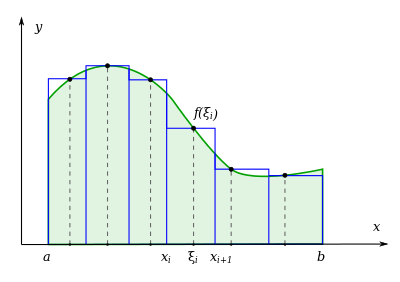
\includegraphics[scale=1.00]{int-stair.png}
\end{figure}

Ясно, что при уменьшении $\Delta \varepsilon_i$ - увеличится точность, так что при устремлении количества подинтервалов в бесконечность, получим точную площадь под функцией.

Можно оценить интеграл т.н. Римановыми суммами, то есть суммами площадей вот таких "лесенок".

Пример:

$$\int _0^1x^2dx = \lim_{n\to\infty}(\frac 1n^2 + \frac 2n ^2 + \ldots + \frac nn^2)=\lim _{n\to\infty}\frac{n(n+1)(2n+1)}{6n^3} = \frac 13$$

Определение интеграла по Риману: 

Пусть функция $f$ определена на отрезке $[a,b]$, $\Delta x = \frac{b-a}n$, $x_i$ - точки, принадлежащие интервалам. Тогда
$$\int _a^b f(x)dx = \lim \Delta x \sum f(x_i)$$

Функция интегрируема по Риману, если такой предел существует и не зависит от $x_i$.

Теорема 1. Если $F$ непрерывна на промежутке от a до b или имеет конечное число отчек разрыва, то $F$ интегрируема по Риману на этом промежутке.

Свойтва интегралов:

$$\alpha \int f(x) + \lambda g(x)dx = \alpha\int f(x)dx + \lambda\int g(x)dx$$

$$\int _a^b f(x)dx = \int _a^cfdx + \int _c^b f(x)dx$$

$$(b-a)max f(x) >\int_a^b f(x)dx>(b-a)min f(x)$$



\end{document}












            






